% $Header: /cvsroot/latex-beamer/latex-beamer/solutions/conference-talks/conference-ornate-20min.en.tex,v 1.7 2007/01/28 20:48:23 tantau Exp $

\documentclass{beamer}
\usepackage{listings}
\lstset{basicstyle=\footnotesize}


% This file is a solution template for:

% - Talk at a conference/colloquium.
% - Talk length is about 20min.
% - Style is ornate.



% Copyright 2004 by Till Tantau <tantau@users.sourceforge.net>.
%
% In principle, this file can be redistributed and/or modified under
% the terms of the GNU Public License, version 2.
%
% However, this file is supposed to be a template to be modified
% for your own needs. For this reason, if you use this file as a
% template and not specifically distribute it as part of a another
% package/program, I grant the extra permission to freely copy and
% modify this file as you see fit and even to delete this copyright
% notice. 


\mode<presentation>
{
  \usetheme{Warsaw}
  % or ...

  \setbeamercovered{transparent}
  % or whatever (possibly just delete it)
}


\usepackage[english]{babel}
% or whatever

%\usepackage[latin1]{inputenc}
% or whatever

%\usepackage{times}
%\usepackage[T1]{fontenc}
% Or whatever. Note that the encoding and the font should match. If T1
% does not look nice, try deleting the line with the fontenc.


\title[Bread Crumb Classification Using Fractal and Multifractal Features] % (optional, use only with long paper titles)
{Bread Crumb Classification Using Fractal and Multifractal Features}

\author
{Rodrigo Baravalle\inst{1} \and Claudio Delrieux\inst{2} \and Juan Carlos G\'omez\inst{1}}
% - Give the names in the same order as the appear in the paper.
% - Use the \inst{?} command only if the authors have different
%   affiliation.

\institute
{
  \inst{1}%
  Laboratorio de Sistemas Din\'amicos y Procesamiento de Informaci\'on. FCEIA, Universidad Nacional de Rosario - CIFASIS - CONICET. \{baravalle,gomez\}@cifasis-conicet.gov.ar
  \and
  \inst{2}%
DIEC, Universidad Nacional del Sur - IIIE-CONICET. cad@uns.edu.ar
}
% - Use the \inst command only if there are several affiliations.
% - Keep it simple, no one is interested in your street address.

\date[Noviembre 2012] % (optional, should be abbreviation of conference name)
% - Either use conference name or its abbreviation.
% - Not really informative to the audience, more for people (including
%   yourself) who are reading the slides online

\subject{Computaci\'on Gr\'afica}
% This is only inserted into the PDF information catalog. Can be left
% out. 



% If you have a file called "university-logo-filename.xxx", where xxx
% is a graphic format that can be processed by latex or pdflatex,
% resp., then you can add a logo as follows:

% \pgfdeclareimage[height=0.5cm]{university-logo}{university-logo-filename}
% \logo{\pgfuseimage{university-logo}}



% Delete this, if you do not want the table of contents to pop up at
% the beginning of each subsection:
%\AtBeginSubsection[]
%{
%  \begin{frame}<beamer>{Outline}
%    \tableofcontents[currentsection,currentsubsection]
%  \end{frame}
%}


% If you wish to uncover everything in a step-wise fashion, uncomment
% the following command: 

%\beamerdefaultoverlayspecification{<+->}


\begin{document}

\begin{frame}
  \titlepage
    \begin{center}
    
\includegraphics[scale=0.08]{cifasislogo}
    \end{center}
\end{frame}

\begin{frame}
%\begin{center}
{\huge Resumen:}
Se presentan resultados de clasificaci\'on sobre muestras de im\'agenes digitalizadas de cortes de pan de distinto tipo. Se realiza una extracci\'on de caracter\'isticas fractales y multifractales, realizando un entrenamiento por medio de Support Vector Machines, alcanzando una tasa de aciertos por encima del $90\%$.
%\end{center}
\end{frame}

\begin{frame}{Esquema de la charla}
  \tableofcontents[pausesections]
  % You might wish to add the option [pausesections]
\end{frame}


% Structuring a talk is a difficult task and the following structure
% may not be suitable. Here are some rules that apply for this
% solution: 

% - Exactly two or three sections (other than the summary).
% - At *most* three subsections per section.
% - Talk about 30s to 2min per frame. So there should be between about
%   15 and 30 frames, all told.

% - A conference audience is likely to know very little of what you
%   are going to talk about. So *simplify*!
% - In a 20min talk, getting the main ideas across is hard
%   enough. Leave out details, even if it means being less precise than
%   you think necessary.
% - If you omit details that are vital to the proof/implementation,
%   just say so once. Everybody will be happy with that.

\section{Introducci\'on}

\subsection{Clasificaci\'on}

\begin{frame}
\begin{center}
{\huge Clasificaci\'on de muestras de pan }\\
\vspace{10px}
{\large \'Util para distinguir im\'agenes de pan sint\'eticas de aquellas que no lo son, es decir, validar im\'agenes de pan como tales}\\
\vspace{10px}
{\large Medida de la calidad de im\'agenes digitalizadas de muestras reales}\\
\end{center}
\end{frame}

\begin{frame}
\begin{center}
{\huge Pasos involucrados: }\\
\begin{itemize}
\item Extracci\'on de caracter\'isticas
\item Construcci\'on del clasificador
\item C\'alculo de resultados (porcentaje de aciertos y errores)
\end{itemize}
\end{center}
\end{frame}

\subsection{Fractales}
\begin{frame}
{\huge Fractales }
\begin{itemize}
\item T\'ermino acu\~nado por el matem\'atico Mandelbrot hacia fines del siglo pasado, para describir elementos naturales o abstractos, que presentan caracter\'isticas de {\em autosimilaridad}.
\item Dimensi\'on Fractal: generalizaci\'on de dimensi\'on euclideana. Usualmente representa la capacidad de un objeto de llenar el espacio en el que est\'a contenido.
\item Multifractal: aquellos elementos cuyas propiedades fractales son diferentes a diferentes escalas
\end{itemize}
\end{frame}


\section{Clasificaci\'on}

\subsection{Base de Datos de im\'agenes de Pan}
\begin{frame}
{\huge Base de Datos de im\'agenes de Pan}
\begin{itemize}
\item $50$ im\'agenes de cuatro tipos diferentes de pan fueron digitalizadas ($200$ im\'agenes en total)
\item Se descargaron $100$ im\'agenes aleatorias de la base de datos CalTech101 (im\'agenes de objetos que no son pan)
\item $20$ im\'agenes de cada tipo de pan fueron obtenidas con una c\'amara digital ($80$ im\'agenes en total)
\begin{figure}
\centering
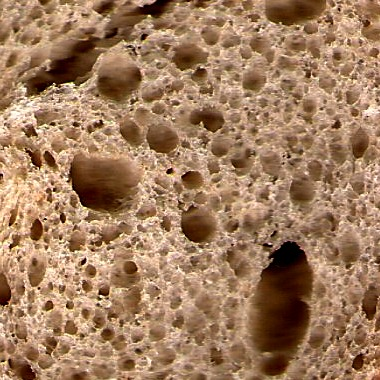
\includegraphics[scale=0.97]{../imagenes/baguette20}
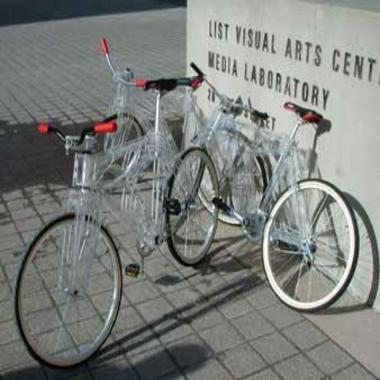
\includegraphics[scale=0.2]{../exps/100sample/res/image_0351}
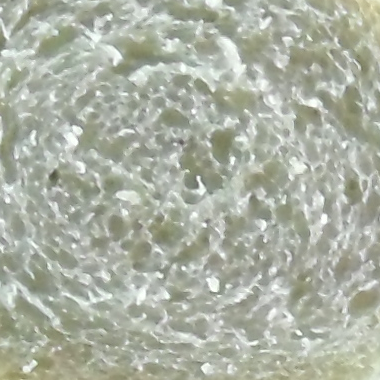
\includegraphics[scale=0.2]{../imagenes/camera/b}
\end{figure}


\end{itemize}
\end{frame}

\subsection{Caracter\'isticas Utilizadas}
\begin{frame}
{\huge Caracter\'isticas Utilizadas}
\begin{itemize}
\item Dimensi\'on Box
\item Dimensi\'on fractal Morfol\'ogica
\item Espectro multifractal ($40$ Features)
    \begin{itemize}
        \item $\alpha$ imagen (caracteriza la regularidad {\em local} de la imagen)
        \item distribuci\'on de valores $\alpha$ en la imagen (caracterizaci\'on {\em global} de la regularidad)
    \end{itemize}
\item Para establecer una comparaci\'on, caracter\'isticas RGB fueron extra\'idas (promedio R, promedio G, promedio B)
\end{itemize}

\end{frame}


\subsection{SVMs}
\begin{frame}
{\huge SVMs}
\begin{center}
\begin{itemize}
\item Proponen un m\'etodo de clasificaci\'on {\em supervisado} (las etiquetas est\'an presentes en la etapa de entrenamiento)
\end{itemize}

\end{center}
\end{frame}

\section{Resultados}

\begin{frame}
{\huge Resultados}
\begin{center}
\begin{table}[htb]
\centering
\begin{tabular}{|c|c|c|c|}
    Features & Fractals & non Fractals & combined\\
    \hline
    Accuracy  & $93.2\%$ & $88.0\%$ & $\textbf{94.4\%}$\\
\end{tabular}
\caption{Results obtained in classification using training and testing samples from the scanner}
\label{table:tableFirstTest}

\begin{table}[ht!b]
\centering
\begin{tabular}{|c|c|c|c|}
    Features & Fractals & non Fractals & combined\\
    \hline
    Accuracy  & $86.5\%$ & $72\%$ & $\textbf{89.5\%}$\\
\end{tabular}
\caption{Results obtained in classification using training and testing samples from the camera and from the scanner}
\label{table:tableRobustnessTest1}
\end{table}
\end{table}

\begin{table}[htb]
\centering
\begin{tabular}{|c|c|c|c|}
    Features & Fractals & non Fractals & combined\\
    \hline
    Accuracy  & $\textbf{50}\%$ & $20\%$ & $45\%$\\
\end{tabular}
\caption{Results obtained when training with a capturing condition and testing with a different one}
\label{table:tableRobustnessTest2}
\end{table}
\end{center}
\end{frame}

\section{Conclusiones}

\begin{frame}{Conclusiones}

\begin{itemize}
\item Las features caracterizan las muestras con muy buena precisi\'on
\item La iluminaci\'on afecta las features multifractales de los distintos tipos de pan
\item Es posible extender el clasificador con m\'as tipos de pan manteniendo una buena clasificaci\'on
\item Las features son buenos discriminadores de imagenes de pan respecto de otros tipos de im\'agenes
\item Caracter\'isticas de color muestran resultados comparables, pero fallan a la hora de detectar im\'agenes de pan respecto de im\'agenes de otras clases
\end{itemize}

\end{frame}

\begin{frame}{Trabajos a Futuro}

\begin{itemize}
\item Aumento de la robustez del m\'etodo
\item Utilizaci\'on de las caracter\'isticas extra\'idas para setear par\'ametros en sistemas de part\'iculas, buscando obtener im\'agenes sint\'eticas con caracter\'isticas similares
\item Utilizaci\'on de Principal Component Analysis (PCA) y Feature Selection, buscando reducir la dimensionalidad de los datos.
\end{itemize}

\end{frame}

\begin{frame}
\begin{center}
{\huge Preguntas?}
\end{center}
\end{frame}

\begin{frame}
\begin{center}
{\huge Gracias!}
\end{center}
\end{frame}


\end{document}


